\chapter{Implementation}
\chapquote{You enter the first room of the mansion and it's completely dark. You stumble around bumping into the furniture, but gradually you learn where each piece of furniture is. Finally, after six months or so, you find the light switch, you turn it on, and suddenly it's all illuminated. You can see exactly where you were. Then you move into the next room and spend another six months in the dark.}{Andrew Wiles}{PBS Interview, After proving Fermat's Last Theorem}

This chapter leads on from the Design chapter and provides further in-depth explanation of the implementation for this project. It is structured as follows:
\begin{itemize}
\item Tech Used
\item Blockchain Interaction with Data Structures
\item Challenges
\item Overview
\end{itemize}
\vfill
\section{Technologies Used}
As stated in the Design chapter, MiniNDN was used in order to emulate a working NDN environment on which to prototype code. This chapter will provide more in-depth insight into the different technologies within MiniNDN and indeed all NDN which were used for this solution.\par 
\subsection{SHA256 Library}
An external sha256 library was initially used in order to create hashed blocks in the Blockchain and in order to be able to do the proof-of-work. However, knowing that this wasn't the focus of the project, the idea was quickly scrapped.
\subsection{ndnsec}
Ndnsec is a command line tool for generating keys and certificates. There are 14 modules in ndnsec. They provide the necessary tools for maintaining NDN private and public keys and certificates for identities. When configuring a testbed to use NLSR-Security, what that actually does is utilize ndnsec in order to create and assign keys and certificates. This is done using predefined commands which generate keys and generate and sign certificates for each identity in a network and then dump the certificates in each identity's local files. The public keys are stored in the PIB and the private keys are stored in the TPM.
\subsection{NLSR Security}
As mentioned in the State of the Art Chapter, NDN - on an experimental level, relies on the Network Manager to choose a security standard. However, MiniNDN has some built in security features. These are found in \textit{../mini-ndn/ndn-cxx/}. The C++ Library with eXperimental eXtensions provides some essential security tools. NLSR security is one way we can configure network security in NDN. NLSR security works in a trust hierarchy. This has many benefits, including being able to identify routers, keys and messages generated by a given routing process in the same network.\cite{053}\par
\begin{figure}[ht]
\centering
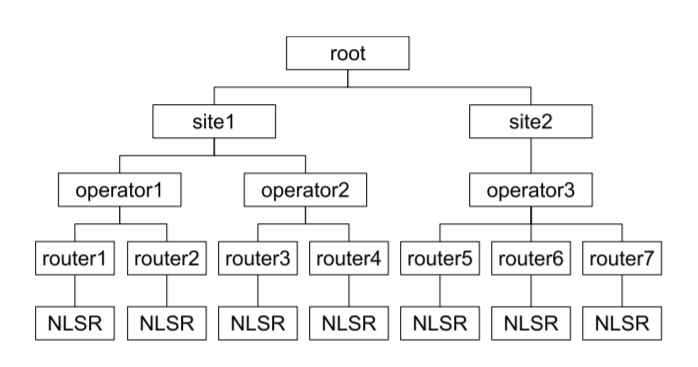
\includegraphics[scale=0.6]{trusthierarchy.png}
\caption{NLSR Trust Hierarchy\cite{054}}
\end{figure}
\vfill
The Trust Model is in place for intra-domain routing and relies on ndnsec to generate keys for NLSR. After some experimentation, it became apparent that NLSR security also imposes on the security protocol to assign a Certificate Authority in order to sign certificates. This is made apparent when printing out the certificates being generated in a long. The difference between having NLSR-Security configured and not shows in the certificates, which have a `self' field which is generated when a certificate is self signed. When NLSR-Security is enabled, these certificates are also replicated with an `NA' field which would normally be populated by the Certificate Authority name. In an experimental environment however, there isn't a specifically assigned CA and this is why this field is populated by `NA'. \par
This security scheme is considered to be hierarchical because NLSR uses a ``five-level hierarchical trust model reflecting the administrative structure"\cite{055} of the network. At the top level, the root or trust anchor, issues certificates to sites. The sites are level two and they can have one or more operators(level three), like the clock example in Chapter 1. Each of these can then produce data, which can be routed by a router(level four), which can be forwarded in an NLSR routing process(level five) which produces LSAs containing the data which must be signed.
\begin{figure}[ht]
\centering
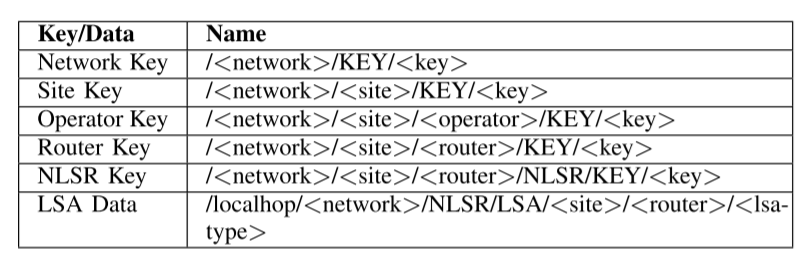
\includegraphics[scale=0.6]{nlsr-sec.png}
\caption{Keys generated with NLSR-Security\cite{056}}
\end{figure}


\section{Component Interaction with Data Structures}
Incorporating the Blockchain Data Structure into the security module of ndn-cxx has been challenging. To a degree because ndn-cxx security is split between version 1 and 2 of the security module. The KeyChain is implemented in v2 but still has a header in v1 and uses the PIB and TPM from v1. There is also the problem of the security modules restarting themselves sporadically.
\subsection{Public Information Base}

The Public Information Base(PIB) is maintained in ndn-cxx. It is instantiated by the KeyChain. The PIB has two backend modules, pib-memory and pib-sqlite3. The PIB sends information to pib-memory which in turn sends information to pib-sqlite3 which in turn stores information in the pib.db. This is where the public keys are stored, i.e. the Public File. The PIB is managed by the KeyChain.

\subsection{The KeyChain}

The KeyChain proved to be very problematic. This is the data structure in charge of instantiating the PIB and creating all certificates in a network, and making sure they are signed. If self-signing is allowed, this is done in the KeyChain class. The KeyChain also compares whether the Trusted Platform Module and the Public Information Base matched and if not, the KeyChain would restart and begin the security process all over again, by getting the PIB and TPM locations, their factories, creating them, then checking if they match again, until they do, and if so, the KeyChain creates the certificates for the network.\par

The problem with the KeyChain and implementing Blockchain begins with its design by the NDN team. The following is a log that was created using the std library as opposed to NDN's boost library approach to making logs. This was done in order to have a separate file to the already very busy NDN log. This log records every time the KeyChain constructor is used. The numbers on the screen represent the Blockchain size. The certificates in the log get printed any time a certificate gets added to the Blockchain. The problem here is that the KeyChain keeps getting instantiated. Because the KeyChain keeps getting reset, we see that the Blockchain is also being reset every time. \par 

This is occurs because of the default security design in the NDN architecture. When MiniNDN is running NLSR-Security, it calls a new instance of the ndnsec tools for every entity. When the new instance is called, and the certgen function is used, that creates a new KeyChain. However, if the TPM and PIB don't match up then the KeyChain gets reset. This means that it is impossible to maintain a Blockchain in the KeyChain class, unless a specific security protocol is designed to run on this system. \par 

The workaround for this has been to dump the PibBlocks into a completely separate data structure or even file in order for the nodes to be able to receive it. This is because the KeyChain class uses smart pointers to initialize PibBlockchains which in turn means that if a KeyChain goes out of scope as it would if it is running the reset() function when the TPM and PIB don't match up, the C++ Compiler simply deletes all references to the Blockchain. \par

A better solution would be to run the Blockchain outside of the security module, so it doesn't keep getting reset and wiped sporadically. 


\begin{figure}
\centering
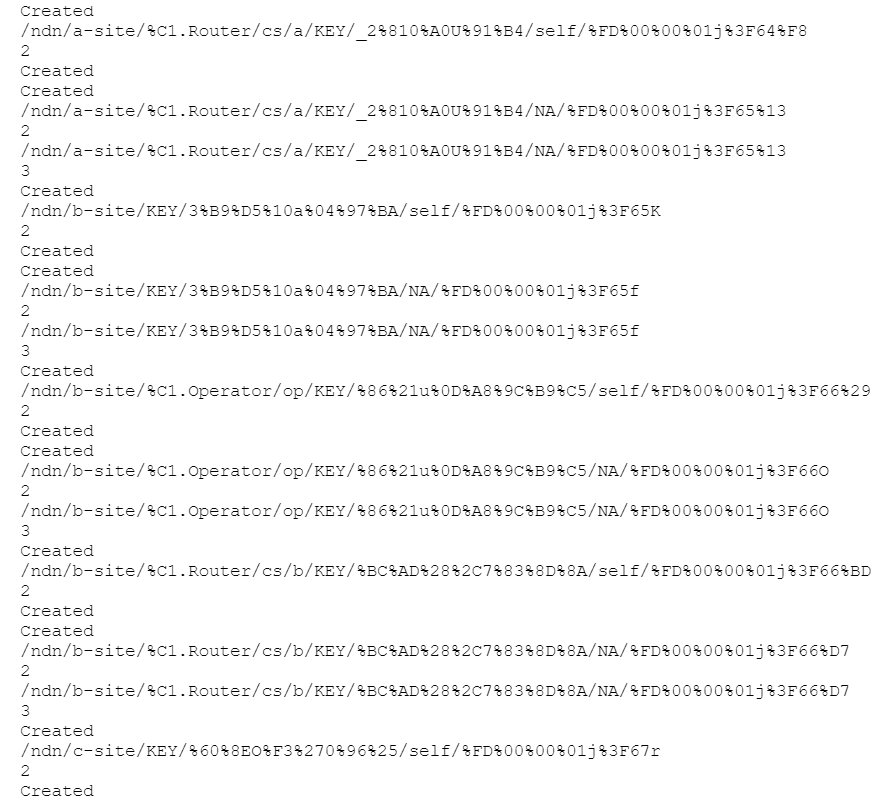
\includegraphics[scale=1]{log.png}
\caption{KeyChain log}
\end{figure}




\section{Challenges}
Most of the design and implementation challenges for this project have been described above. To summarize, the two main challenges are communicating the Blockchain to all of the nodes in a network, and also appending the Blockchain class to the security library without recalling its constructor constantly, the way KeyChain does. These issues are solved by writing a wrapper for the PibBlockchain class, and also, upon limited trial, selecting the Chronosync approach in the dissemination of the Blockchain. 
